\chapter{Introduction}

\section{Project summary}
This project focuses on developing a system that can survey an area of the sea from inputs in a UI autonomously, thus removing the need for route planning by surveyors, enabling them to focus on data analysis rather than data acquisition. 

\subsection{Motivation}
In recent years, there has been an increased focus on autonomous vehicles, both by land, sea, and air. Self-driving cars, drones, and automatic survey vessels are examples of this, and the trend seems to continue as the technology matures and becomes accepted more broadly in society.

Autonomy ensures repeatability, reduces many categories of risk, and - by definition - eliminates the error-prone human element from the equation, often leading to much better results and favourable cost.
 
\section{System description}

An overview of the system is seen in figure~\ref{fig:rich_image}.

As such, the system requires a number of components. 

A UI which allows the user to set up parameters such as the width of the survey equipment, and specify an area on a map to cover in an intuitive way. The map will be updated continually if a network is available, otherwise an offline version of the most important quadrants is used.

A controller which takes care of navigation and autopiloting based on user commands, parameters, and GPS data. Relevant information such as position of the ship, planned route, and completed route are then shown in the UI.

A server which hosts the website and writes/reads data to/from the website and controller.

A prototype ship with a rudder and thruster and hull space for the controller unit, GPS, battery, motor controller(s).

A command computer to communicate with the controller and view the UI.

The general sequence diagram in figure~\ref{fig:general_sd} describes the general flow and functionality of the system.

\begin{figure}[H]
	\centering
	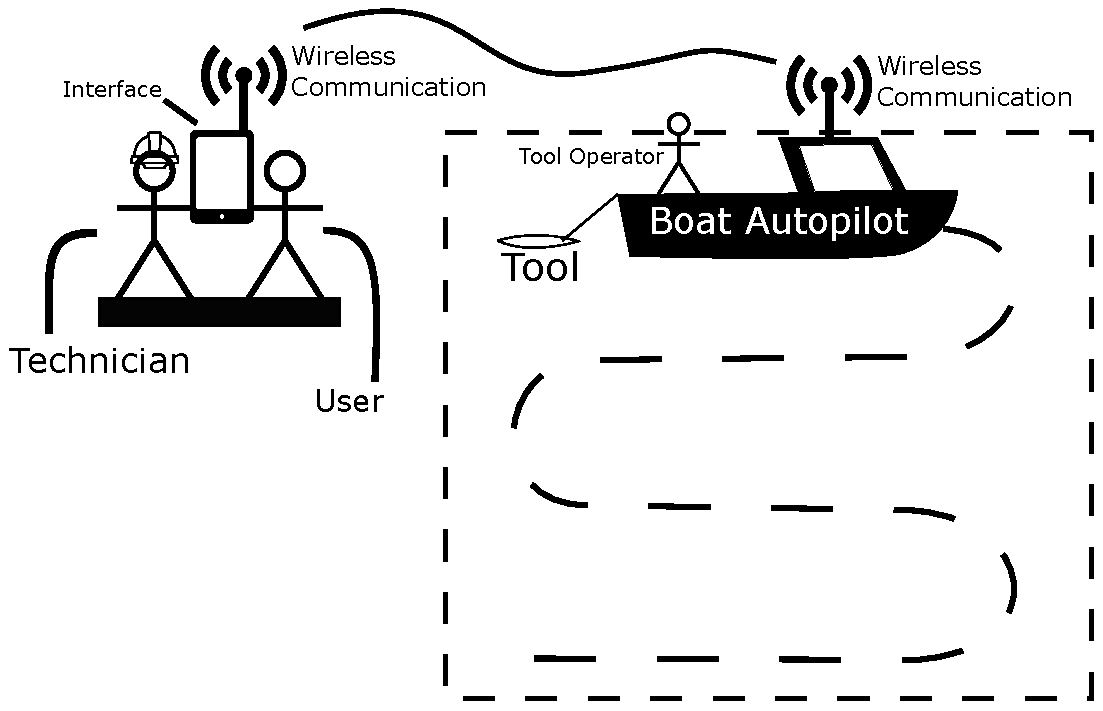
\includegraphics[width=1\linewidth]{Images/Introduction/rich_image}
	\caption{Rich image}
	\label{fig:rich_image}
\end{figure}

\begin{figure}[H]
	\centering
	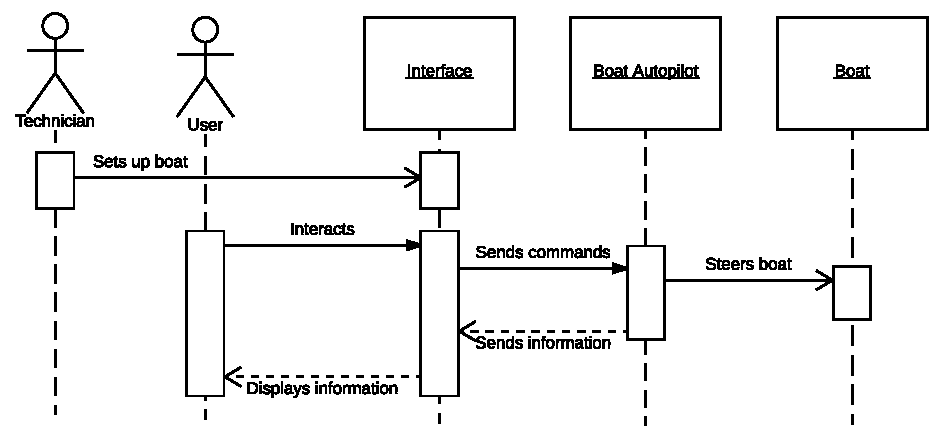
\includegraphics[width=1\linewidth]{Images/Introduction/General_SD}
	\caption{General sequence diagram}
	\label{fig:general_sd}
\end{figure}

The project details are taken from the project offer on blackboard\cite{problem-description} which was used in the early phases of the project.

The market for unmanned surface vessels (sailing drones) is growing, and there is a need for an open architecture auto-pilot that is usable on different platforms.

This project is about designing and implementing the electronics and embedded software for an autopilot which is able to receive steering commands from a navigation system (distance to go left/right) and from thoes instructions, steer a small boat (et. control left/right thrusters).

\paragraph{Project details}
\begin{itemize}
\item PCB design of autopilot electronics (if something existing cannot be used)
\item Implement PID control loop to get back on course based on received left/right commands
\item Control of thrusters in case of two-thruster catamaran
\item Control of wheel in case of outboard motor on boat
\item Test trials at sea
\item EIVA will provide necessary hardware, include test boats / catamarans, including PCB production cost
\item EIVA will provide work-space (desk, lunch etc) at EIVA's facilities
\item IF the project is successful, EIVA will offer to finalise the product and make it available for sale with a commision to the student
\end{itemize}

The requirements for the project are based on these bullet points from EIVA's boat autopilot project details on blackboard, but due to lack of communication and differing perspectives, the project requirements were finalized by the group itself, and not by EIVA. The requirements are specified in the following section.
